\documentclass{article}

\usepackage{graphicx}
\usepackage{cprotect}  % Used for verb inside caption
\usepackage{siunitx}  % Render SI-units nice and easy
\usepackage{listings}  % Used to show code
\usepackage{color}

\author{Tora Dahl}
\author{Thorvald Ballestad}
\title{Reproducing the classical pong game}

%% Settings for listings (code) - shamelessly copied from wikibooks %%
\definecolor{mygreen}{rgb}{0,0.6,0}
\definecolor{mygray}{rgb}{0.5,0.5,0.5}
\definecolor{mymauve}{rgb}{0.58,0,0.82}
\lstset{ 
  backgroundcolor=\color{white},   % choose the background color; you must add \usepackage{color} or \usepackage{xcolor}; should come as last argument
  basicstyle=\footnotesize,        % the size of the fonts that are used for the code
  breakatwhitespace=false,         % sets if automatic breaks should only happen at whitespace
  breaklines=true,                 % sets automatic line breaking
  captionpos=b,                    % sets the caption-position to bottom
  commentstyle=\color{mygreen},    % comment style
  escapeinside={\%*}{*)},          % if you want to add LaTeX within your code
  extendedchars=true,              % lets you use non-ASCII characters; for 8-bits encodings only, does not work with UTF-8
  frame=single,	                   % adds a frame around the code
  keepspaces=true,                 % keeps spaces in text, useful for keeping indentation of code (possibly needs columns=flexible)
  keywordstyle=\color{blue},       % keyword style
  language=C++,                    % the language of the code
  morekeywords={*,...},            % if you want to add more keywords to the set
  numbers=left,                    % where to put the line-numbers; possible values are (none, left, right)
  numbersep=5pt,                   % how far the line-numbers are from the code
  numberstyle=\tiny\color{mygray}, % the style that is used for the line-numbers
  rulecolor=\color{black},         % if not set, the frame-color may be changed on line-breaks within not-black text (e.g. comments (green here))
  showspaces=false,                % show spaces everywhere adding particular underscores; it overrides 'showstringspaces'
  showstringspaces=false,          % underline spaces within strings only
  showtabs=false,                  % show tabs within strings adding particular underscores
  stepnumber=2,                    % the step between two line-numbers. If it's 1, each line will be numbered
  stringstyle=\color{mymauve},     % string literal style
  tabsize=2,	                   % sets default tabsize to 2 spaces
  title=\lstname                   % show the filename of files included with \lstinputlisting; also try caption instead of title
}

\begin{document}
\maketitle

\begin{abstract}
  We attemptet reproducing the classical pong game using an Arduino and a 32x32 pixel LED display.
\end{abstract}

\section{Vision}
The initial idea was to create a pong game.
The pong game is an arcade classic.
Released in 1972 it was one of the first arcade video games created.
The game is between two players.
Each player controls a paddle which can be moved up or down.
A ball bounces back and forth, and the players has to hit the ball using the paddle.
A player gains a point when the opponent fails to return the ball.\\

We wished to use a low-pixel display for the project, controlled by an Arduino.
The paddles needed some type of control, in the first iteration the idea was to use a simple potentiometer.
This input could be made more sophisticated in later iterations.

\section{Results}
The game is run on an Arduino Uno.

As monitor, a 32x32 RGB LED Matrix Panel from Adafruit, product id 607, was used.
Each of the 1024 pixels has a RGB LED pixel, using the Arduino one gets 12-bit color depth.

For user input voltage measurements from simple potentiometers where used.

\subsection{Interfacing the display}
The first challenge is interfacing the display.
On Adafruits homepage there are thorough guides to doing this.
The display features a 16 pin connector, the pinout is shown in figure \ref{fig:pinout}.
\begin{figure}[h]
  \centering
  \includegraphics[width=.75\textwidth]{media/pinout}
  \cprotect\caption{Pinout of connector on the 32x32 display. Note that this is the male connect, mounted on the display itself. Diagram created by Phillip Burges, distributed on Adafruit's homepage under the filename \verb|led_matrix_socket2.png|.}
  \label{fig:pinout}
\end{figure}

To reliably connect the display to the Arduino, a cutom shield was created using Arduino's proto shield.
This proved to be very advanteagous over simply using jumper cables -- it allowed for easily connecting and disconneting the display, and also minimized cables coming loose as a potential source of error.
Table \ref{tab:pinout} shows how the display was connected to the Arduino.

\begin{table}[h]
  \centering
  \begin{tabular}{ll}
    Display& Arduino\\\hline
    R1& 2\\
    G1& 3\\
    B1& 4\\
    R2& 5\\
    G2& 6\\
    B2& 7\\
    CLK& 8\\
    OE& 9\\
    LAt& 10\\
    A& A0\\
    B& A1\\
    C& A2\\
    D& A3\\
    GND& GND
  \end{tabular}
  \caption{Table explaining the circuit between the 32x32 display and the Arduino. Arduino pins with only a number refers to the digital pins, pins prefixed with ``A'' refers to analog pins. See figure \ref{fig:pinout} for the pinout of the display connector.}
  \label{tab:pinout}
\end{table}

\begin{figure}[h]
  \centering
  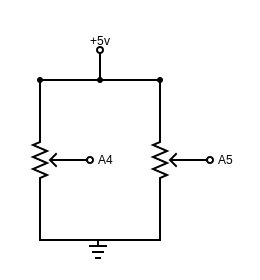
\includegraphics[width=.75\textwidth]{media/input2}
  \caption{User input circuit. A4 and A5 refers to the analog input pins on the Arduino.}
  \label{fig:input}
\end{figure}

\subsection{Software}
\begin{lstlisting}
#include <RGBmatrixPanel.h>

#define CLK  8
#define OE   9
#define LAT 10
#define A   A0
#define B   A1
#define C   A2
#define D   A3

RGBmatrixPanel matrix(A, B, C, D, CLK, LAT, OE, false);

int rate = 50;
const int WIDTH = 31;
const int HEIGHT = 31;

/*******
* PONG *
*******/
float BALL_SPEED = 1;
int POINTS_TO_WIN = 3;
float BAR_SPEED = 1.8;

// NB. Initial pos 0 and positive velocity will fuck it up
// (No way that it can reach the state x=0, vx>0, so this is an impossible initial state).
float x = 1;
float y = 1;
float vx = sin(1)*BALL_SPEED;
float vy = cos(1)*BALL_SPEED;

float bar1 = 16;
float bar2 = 16;

int bar1_x = 1;
int bar2_x = 30;

int bar_height = 2;

int points_1 = 0;
int points_2 = 0;

void reset_pong() {
  reset();

  bar1 = 16;
  bar2 = 16;

  points_1 = 0;
  points_2 = 0;
}

void control_bar(float &bar) {
  bar = min(HEIGHT-bar_height, bar);
  bar = max(bar_height, bar);
}

void game_won() {
  matrix.fillScreen(0);
  for (int i = 0; i < WIDTH/2; i++) {
    matrix.fillCircle(WIDTH/2, HEIGHT/2, i, matrix.Color333(7,0,0));
    delay(50);
  }
  
  matrix.setCursor(3, 6);
  matrix.setTextSize(0.5);
  matrix.setTextColor(matrix.Color333(7,7,7));
  matrix.print("Game over!");
  delay(3000);
}

void reset() {
  // Resets game
  // Sets balls velocity in x-direction
  // to between 50 and 100 percent of BALL_SPEED
  // sets y to be such that total speed is BALL_SPEED
  x = int(WIDTH/2);
  y = int(HEIGHT/2);
  vx = random(50, 100)*BALL_SPEED/100.0;
  vy = sqrt(sq(BALL_SPEED)-sq(vx));
  int signx = random(-10, 10) > 0? -1 : 1;
  int signy = random(-10, 10) > 0? -1 : 1;
  vx *= signx;
  vy *= signy;
  draw();
}

void draw() {

  matrix.fillScreen(matrix.Color333(0, 0, 0));
  matrix.drawPixel((int) x, (int) y, matrix.Color333(4, 0, 0));
  matrix.drawLine(bar1_x, int(bar1) - bar_height, bar1_x, int(bar1) + bar_height, matrix.Color333(4, 4, 4));
  matrix.drawLine(bar2_x, int(bar2) - bar_height, bar2_x, int(bar2) + bar_height, matrix.Color333(4, 4, 4));

  matrix.setCursor(10, 0);
  matrix.setTextSize(0.5);
  matrix.setTextColor(matrix.Color333(0,7,0));
  matrix.print(points_1);
  matrix.setCursor(20, 0);   // start at top left, with one pixel of spacing
  matrix.print(points_2);

}

void pong() {
  reset_pong();
  while(true) {
    /***********
     * Measure *
     ***********/
    int sensorValue1 = analogRead(A4);
    int sensorValue2 = analogRead(A5);
    float voltage1 = sensorValue1 * (5.0 / 1023.0);
    float voltage2 = sensorValue2 * (5.0 / 1023.0);

    /********
     * Draw *
     ********/
    draw();

    /**************
     * Game logic *
     **************/

    float delta_bar1 = (2.5 - voltage1)/2.5;
    float delta_bar2 = (2.5 - voltage2)/2.5;
    bar1 += abs(delta_bar1)<0.3 ? 0 : delta_bar1*BAR_SPEED;
    bar2 += abs(delta_bar2)<0.3 ? 0 : delta_bar2*BAR_SPEED;
    control_bar(bar1);
    control_bar(bar2);

    // Check collision with bar
    if (int(x) <= bar1_x and bar1 + bar_height >= y and bar1 - bar_height <= y) {
      vx = abs(vx);
    }

    if (int(x) >= bar2_x and bar2 + bar_height >= y and bar2 - bar_height <= y) {
      vx = -abs(vx);
    }

    // Check collison with top or bottom wall, reflect ball
    if (y <= 0 or y >= HEIGHT) {
      vy = -vy;
    }

    // Check collision with end walls, add points
    if (x <= 0){
      points_2++;
      reset();
      delay(400);
    }
    if(x >= WIDTH){
      points_1++;
      reset();
    }

    x += vx;
    y += vy;

    if(points_1==POINTS_TO_WIN or points_2==POINTS_TO_WIN){
      game_won();
      break;
    }

    delay(rate);
  }
}

void setup() {
  matrix.begin();
}

void loop() {
  while(true){
  matrix.fillScreen(0);
  matrix.setCursor(6, 2);
  matrix.print("Menu");
  matrix.fillRect(6, 15, 9, 9, matrix.Color333(4,4,4));
  matrix.fillRect(19, 15, 9, 9, matrix.Color333(4,4,4));
  matrix.fillCircle(10, 19, 2, matrix.Color333(7,0,0));
  matrix.drawLine(20, 22, 25, 16, matrix.Color333(0, 7, 0));
  matrix.drawPixel(26, 16, matrix.Color333(7, 0, 0));
  int x = analogRead(A4)* (5.0 / 1023.0)*6;
  int y = analogRead(A5)* (5.0 / 1023.0)*6;
  matrix.fillCircle(x, y, 1, matrix.Color333(0,0,7));
  delay(5000);
  if(6<x<15){
  pong();}
  delay(40);
}}
\end{lstlisting}

\subsection{Full list of parts}
Finally, here is a complete list of parts used.
\begin{itemize}
\item 32x32 RGB LED Matrix Panel from Adafruit, product id 607.
\item Arduino Uno
\item Arduino Proto shield (Uno size)
\item Two \SI{10}{\kilo\ohm} potentiometers
\item A black metal plate scavenged from an old computer casing
\end{itemize}
The total cost of the parts was zero NOK, as all the parts where found on the lab.
\end{document}
